\documentclass[a4paper,11pt]{book}
\renewcommand{\familydefault}{\sfdefault}

\usepackage{standalone}
\usepackage[english]{babel}
\usepackage[top=3cm]{geometry}
\usepackage{float}
\usepackage{tabularx}
\usepackage{multirow}
\usepackage{booktabs}
\usepackage{pgfplots}
\usepackage{amsmath}
\usepackage{amssymb}
\usepackage{amsfonts}
\usepackage{siunitx}
\usepackage{tikz}
\usepackage{graphics} % for pdf, bitmapped graphics files
\usepackage{graphicx}
\usepackage{exsheets}
\usepackage{algorithm}
\usepackage{algorithmicx}
\usepackage[noend]{algpseudocode}
\usepackage{hyperref}
\usepackage{enumitem}
\usepackage{filecontents}
\usepackage{multirow}
%\usepackage{showframe}% to show frames
%\ifCLASSOPTIONcompsoc
\usepackage[caption=false, font=normalsize, labelfont=sf, textfont=sf]{subfig}
%\else
%\usepackage[caption=false, font=footnotesize]{subfig}
%\fi    

\usetikzlibrary{patterns,arrows,arrows.meta,calc,intersections,shapes,positioning,decorations.pathreplacing,decorations.markings,decorations.pathmorphing}
\usepackage{multicol}

\sisetup{output-decimal-marker={,},exponent-product=\cdot}

\DeclareSIUnit\atm{atm}
\DeclareSIUnit\dioptre{D}



\def\BState{\State\hskip-\ALG@thistlm}


\definecolor{TitleColor}{rgb}{0.65,0.04,0.07}
\definecolor{NumberColor}{rgb}{0.02,0.04,0.48}

\DeclareInstance{exsheets-heading}{fancy}{default}{
toc-reversed = true ,
indent-first = true ,
vscale = 2 ,
pre-code = \IfInsideQuestionT{\rule{\linewidth}{1pt}} ,
post-code =\IfInsideQuestionT{\rule{\linewidth}{1pt}} ,
subtitle-format = \large\scshape\color{rgb:red,0.65;green,0.04;blue,0.07} ,
number-format = \large\bfseries\color{rgb:red,0.02;green,0.04;blue,0.48} ,
points-format = \itshape ,
join = { number[r,B]title[l,B](.333em,0pt);
title[r,B]subtitle[l,B](1em,0pt)
} ,
attach =
{
main[hc,vc]number[hc,vc](0pt,0pt) ;
main[l,vc]subtitle[hc,vc](\marginparsep,0pt)
}
}



\DeclareInstance{exsheets-heading}{block-subtitle}{default}{
vscale = 2 ,
pre-code = \rule{\linewidth}{1pt} ,
post-code = \rule{\linewidth}{1pt} ,%title-format = \large\scshape\color{TitleColor} ,
number-format = \large\bfseries\color{rgb:red,0.02;green,0.04;blue,0.48} ,
subtitle-format = \large\scshape\color{black} ,
join = {
title[r,B]number[l,B](.333em,0pt) ;
title[r,B]subtitle[l,B](1em,0pt)
} ,
attach = {
main[l,vc]title[l,vc](0pt,0pt) ;
main[r,vc]points[l,vc](\marginparsep,0pt)
},
}

\DeclareQuestionClass{textbook}{textbooks}

\SetupExSheets{
  headings = fancy,
  question/print = true ,
  solution/print = false }
 % counter-format = se.qu ,
%  counter-within = section ,
  %question/pre-hook = \rule{\textwidth}{1pt},


\hypersetup{
	colorlinks = true, 
	breaklinks = true, 
	bookmarks = true,
	bookmarksnumbered = true,
	urlcolor = blue, 
	linkcolor = blue, 
	citecolor=blue,
	linktoc=page, 
	pdftitle={}, 
	pdfauthor={\textcopyright Author}, 
	pdfsubject={}, 
	pdfkeywords={}, 
	pdfcreator={pdfLaTeX}, % PDF Creator
	pdfproducer={IEEE} }





\tikzset{point/.style={circle,fill,black!80,inner sep=0pt,minimum size=#1,opacity=0.9}}
\tikzset{point/.default=3pt}\tikzset{vector/.style={line width=1pt,postaction={decorate,decoration={markings,mark=at position 1 with {\arrow{latex}}}}}}
\tikzset{block/.style={rectangle,fill=black!30,draw,minimum size=#1,opacity=0.9,align=center}}
\tikzset{block/.default=15pt}\tikzset{ball/.style={circle,fill=black!30,draw,minimum size=#1,opacity=0.9}}
\tikzset{ball/.default=5pt}\tikzset{pulley/.style={draw=black,line width=0.2pt,circle,minimum size=#1,inner sep=0pt,fill=black!10}}
\tikzset{pulley/.default=20pt}\tikzset{rod/.style={line width=2pt}}
\tikzset{rope/.style={line width=1pt}}
\tikzset{spring/.style={decorate,decoration={coil,amplitude=5pt,segment length=#1,aspect=0.3}}}
\tikzset{spring/.default=5pt}\tikzset{wall/.style={black!10,pattern=north east lines,opacity=0.3}}
\tikzset{ray/.style={line width=0.8pt,postaction={decorate,decoration={markings,mark=at position 0.5 with {\arrow{>}}}}}}
\tikzset{arrow/.style={-latex}}
\tikzset{object/.style={line width=1pt,orange,-latex}}
\tikzset{image/.style={line width=1pt,blue,-latex}}
\tikzset{doublearrow/.style={<->,>=latex,thick}}
\tikzset{brace/.style={decorate,decoration={brace,amplitude=#1}}}
\tikzset{brace/.default=5pt}




\graphicspath{{images/}} 




\makeatletter
\@addtoreset{question}{section}
\makeatother


\begin{document}
\author{Dr. Muhammed Rushdi \and Asem Alaa}

\title{Measurements and Instrumentation [SBE206A] (Fall 2018)\\ Tutorial 2}

\maketitle

\chapter*{Instrument types and performance characteristics}

\begin{itemize}
\item Review of instrument types
\begin{itemize}
\item Active and passive instruments.
\item Null-type and deflection-type instruments.
\item Analogue and digital instruments.
\item Indicating instruments and instruments with a signal output.
\item Smart and non-smart instruments.
\end{itemize}
\item Static characteristics of instruments.
\begin{itemize}
\item Accuracy and inaccuracy (measurement uncertainty).
\item Precision/repeatability/reproducibility.
\item Tolerance.
\item Range or span.
\item Linearity.
\item Sensitivity of measurement.
\item Threshold.
\item Resolution.
\item Sensitivity to disturbance.
\item Hysteresis effects.
\item Dead space.
\end{itemize}
\end{itemize}



\begin{question}
The following resistance values of a platinum resistance thermometer were measured at a range
of temperatures.
 Determine the measurement sensitivity of the instrument in ohms/$^{\circ}$C. \\ \\
\begin{tabular}{cc}
\hline 
Resistance ($\Omega$) & Temperature ($^{\circ}$C) \\ 
\hline 
307 & 200 \\ 
314 & 230 \\ 
321 & 260 \\ 
328 & 290 \\ 
\end{tabular} 
\examspace*{5em}

\end{question}
\begin{solution}


\end{solution}


\begin{question}
A spring balance is calibrated in an environment at a temperature of 20 $^{\circ}$C and has the
following deflection/load characteristic. \\ \\

\begin{tabular}{ccccc}
\hline 
Load (Kg) & 0 & 1 & 2 & 3 \\ 
Deflection (mm) & 0 & 20 & 40 & 60 \\ 
\hline 
\end{tabular}  \\ \\

It is then used in an environment at a temperature of 30 $^{\circ}$C and the following deflec-
tion/load characteristic is measured. \\ \\

\begin{tabular}{ccccc}
\hline 
Load (Kg) & 0 & 1 & 2 & 3 \\ 
Deflection (mm) & 5 & 27 & 49 & 71 \\ 
\hline 
\end{tabular}  \\ \\


Determine the zero drift and sensitivity drift per $^{\circ}$C change in ambient temperature.


\examspace*{5em}

\end{question}
\begin{solution}


\end{solution}


\begin{question}
What is meant by: \\
\begin{itemize}
\item active instruments 
\item passive instruments
\end{itemize}

Give examples of each and discuss the relative merits of these two classes of instruments
\examspace*{5em}

\end{question}
\begin{solution}


\end{solution}


\begin{question}
Discuss the advantages and disadvantages of null and deflection types of measuring instru-
ment. What are null types of instrument mainly used for and why?

\examspace*{5em}

\end{question}
\begin{solution}


\end{solution}


\begin{question}
Explain the difference between accuracy and precision in an instrument.

\examspace*{5em}

\end{question}
\begin{solution}


\end{solution}

\begin{question}
Define sensitivity drift and zero drift. What factors can cause sensitivity drift and zero drift
in instrument characteristics?
\examspace*{5em}

\end{question}
\begin{solution}


\end{solution}

\begin{question}
Define sensitivity drift and zero drift. What factors can cause sensitivity drift and zero drift
in instrument characteristics?
\examspace*{5em}

\end{question}
\begin{solution}


\end{solution}


\begin{question}
A tungsten thermocouple has an output e.m.f. as shown in the following table when its hot
(measuring) junction is at the temperatures shown. Determine the sensitivity of measurement
for the thermocouple in mV/ $^{\circ}$ C.
\\ \\

\begin{tabular}{ccccc}
\hline 
mV & 4.37 & 8.74 & 13.11 & 17.48 \\ 
$^{\circ}$ C & 250 & 500 & 750 & 1000 \\ 
\hline 
\end{tabular}  \\ \\

\examspace*{5em}

\end{question}
\begin{solution}


\end{solution}



\begin{question}
\begin{enumerate}
\item An instrument is calibrated in an environment at a temperature of 20 $^{\circ}$C and the following
output readings y are obtained for various input values x: \\ \\
\begin{tabular}{ccccccc}
\hline 
y & 13.1 & 26.2 & 39.3 & 52.4 & 65.5 & 78.6 \\ 
x & 5 & 10 & 15 & 20 & 25 & 30 \\ 
\hline 
\end{tabular}  \\ \\
Determine the measurement sensitivity, expressed as the ratio $y/x$.

\item When the instrument is subsequently used in an environment at a temperature of 50 $^{\circ}$C,
the input/output characteristic changes to the following: \\ \\ 
\begin{tabular}{ccccccc}
\hline 
y & 14.7 & 29.4 & 44.1 & 58.8 & 73.5 & 88.2 \\ 
x & 5 & 10 & 15 & 20 & 25 & 30 \\ 
\hline 
\end{tabular}  \\ \\
Determine the new measurement sensitivity. Hence determine the sensitivity drift due to
the change in ambient temperature of 50 $^{\circ}$C.
\end{enumerate}

\examspace*{5em}

\end{question}
\begin{solution}

\end{solution}


\begin{question}
A load cell is calibrated in an environment at a temperature of 21 $^{\circ}$C and has the following
deflection/load characteristic: \\ \\

\begin{tabular}{cccccc}
\hline 
Load (Kg) & 0 & 50 & 100 & 150 & 200 \\ 
Deflection (mm) & 0.0 & 0.1 & 0.2 & 0.3 & 0.4 \\ 
\hline 
\end{tabular}  \\ \\

When used in an environment at 35 $^{\circ}$C, its characteristic changes to the following: \\ \\

\begin{tabular}{cccccc}
\hline 
Load (Kg) & 0 & 50 & 100 & 150 & 200 \\ 
Deflection (mm) & 0.2 & 1.3 & 2.4 & 3.5 & 4.6 \\ 
\hline 
\end{tabular} \\ \\

\begin{enumerate}
\item Determine the sensitivity at 21 $^{\circ}$C and 35 $^{\circ}$C.
\item Calculate the total zero drift and sensitivity drift at $^{\circ}$C.
\item Hence determine the zero drift and sensitivity drift coefficients (in units of μm/ $^{\circ}$C and
(μm per kg)/($^{\circ}$C)).
\end{enumerate}

\examspace*{5em}

\end{question}
\begin{solution}


\end{solution}


\begin{question}
An unmanned submarine is equipped with temperature and depth measuring instruments
and has radio equipment that can transmit the output readings of these instruments back to
the surface. The submarine is initially floating on the surface of the sea with the instrument
output readings in steady state. The depthmeasuring instrument is approximately zero order
and the temperature transducer first order with a time constant of 50 seconds. The water
temperature on the sea surface, $T_0$ , is 20 $^{\circ}$C and the temperature $T_x$ at a depth of x metres is
given by the relation:
$T_x$ = $T_0$ − 0.01x

\begin{enumerate}
\item If the submarine starts diving at time zero, and thereafter goes down at a velocity of 0.5
metres/second, draw a table showing the temperature and depth measurements reported at
intervals of 100 seconds over the first 500 seconds of travel. Show also in the table the error
in each temperature reading.
\item  What temperature does the submarine report at a depth of 1000 metres?
\end{enumerate}

\examspace*{5em}

\end{question}
\begin{solution}


\end{solution}


\begin{question}
Write down the general differential equation describing the dynamic response of a second
order measuring instrument and state the expressions relating the static sensitivity, undamped
natural frequency and damping ratio to the parameters in this differential equation. Sketch
the instrument response for the cases of heavy damping, critical damping and light damping,
and state which of these is the usual target when a second order instrument is being designed.

\examspace*{5em}

\end{question}
\begin{solution}


\end{solution}


\begin{figure*}[h!]\label{fig:comparison}
   
  \subfloat[]{
       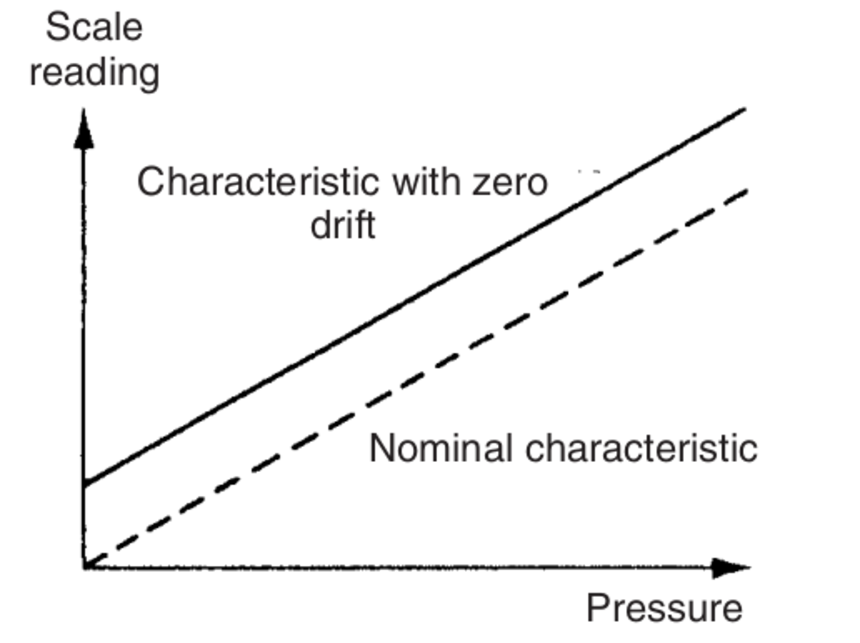
\includegraphics[width=0.40\linewidth]{zdrift}
       }
    \label{fig:zdrift}\hfill
  \subfloat[]{
        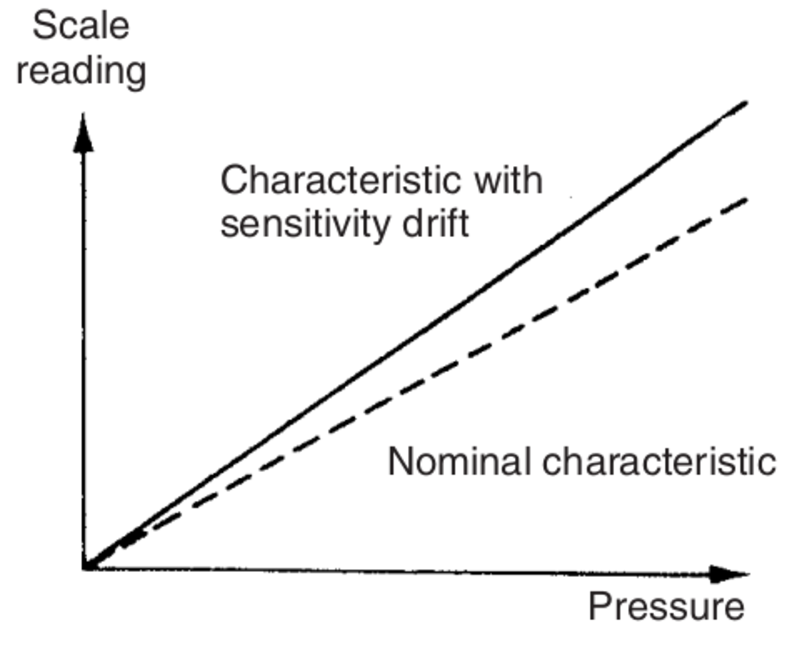
\includegraphics[width=0.40\linewidth]{sdrift}
        }
    \label{fig:sdrift}\\
  \subfloat[]{
       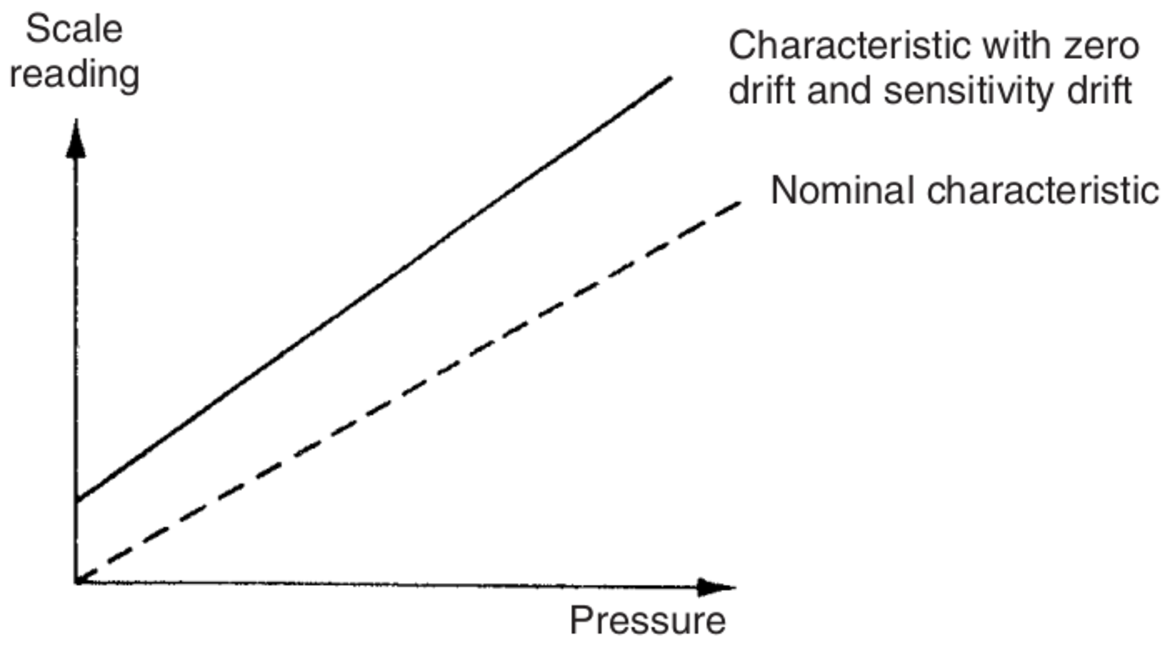
\includegraphics[width=0.40\linewidth]{zsdrift}
        }
   \label{fig:zsdrift}\hfill
  \caption{ Comparison between (a) zero-dirft (b) sensitivity-drift (c) zero- and sensitivity-drift.} 
\end{figure*}

\begin{figure*}[h!]\label{fig:comparison}
  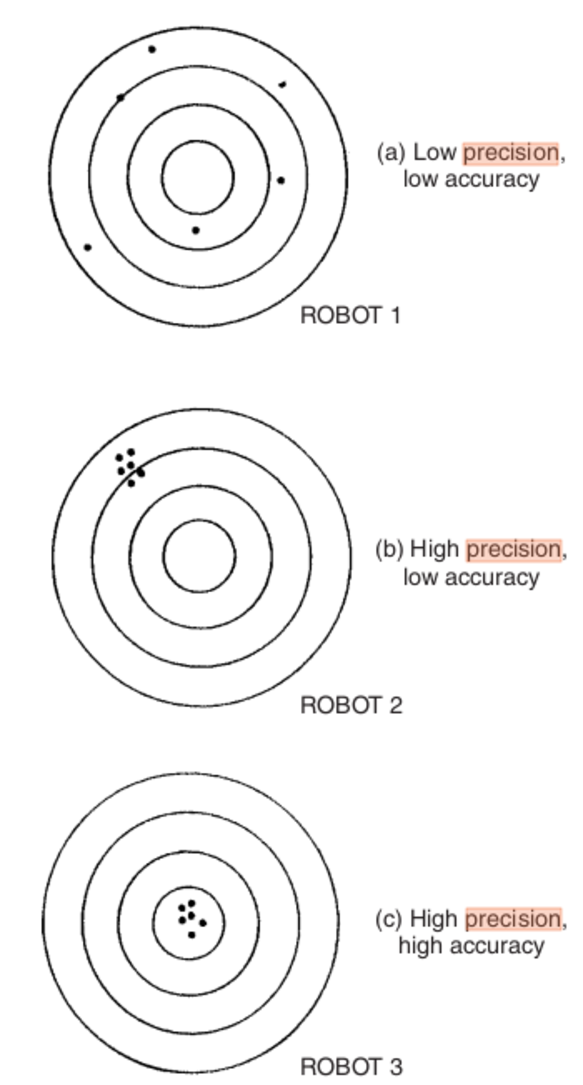
\includegraphics[width=0.40\linewidth]{acc_precision}
  \caption{ Comparison between accuracy and precision.} 
\end{figure*}

\end{document}
